\documentclass{TDP005mall}
\usepackage{float}
\newcommand{\version}{Version 1.1}
\author{David Dumminsek, \url{davdu153@student.liu.se}\\
  Haris Basic, \url{harba466@student.liu.se}\\
  }
\title{Kravspecifikation}
\date{2022-11-15}
\rhead{David Dumminsek\\
Haris Basic\\
}

\begin{document}
\projectpage
\section{Revisionshistorik}
\begin{table}[!h]
\begin{tabularx}{\linewidth}{|l|X|l|}
\hline
Ver. & Revisionsbeskrivning & Datum \\\hline
1.0 & Första utkastet för kravspecifikation inlämnad & 2022-11-15 \\\hline
1.1 & Rättning efter feedback & 2022-11-28 \\\hline
\end{tabularx}
\end{table}
\tableofcontents
\clearpage
\section{Dogeater: The Goblin Ace}

Ett ''bullet hell'' spel där luftstrider utkämpas mellan huvudkaraktären Dogeater, som är en så kallad goblin, samt en stor mängd fientliga flygplan.
Spelet utspelar sig i en tvådimensionell värld som betraktas med fågelperspektiv.

\subsection{Spelidé}
Spelet kommer vara ett klassiskt ''bullet hell'' spel där spelaren behöver undvika en stor mängd projektiler och fiender tills slutet av banan har nåtts. 
Spelaren kommer styra ett stridsflygplan i en vertikalt skrollande värld.

Fiender kommer skapas och långsamt visa sig när banan har skrollat upp till dem. Det kommer finnas flera olika fiendetyper med olika rörelse- och attackmönster. 
Fienderna kommer avfyra skadliga projektiler som spelaren behöver undvika. Då en projektil kolliderar med spelaren så förlorar spelaren ett liv.
Om spelaren skulle få slut på liv och sedan dö ytterligare en gång så börjar spelaren om från första banan.
När spelaren nått slutet på banan så skickas spelaren till nästa bana.
Spelaren har möjlighet att skjuta projektiler som vid kollision med fientliga enheter skadar de och eventuellt dödar de om de tagit tillräckligt med skada.
Vid eliminering av fiender får spelaren poäng som sedan kan omvandlas till nya liv då tillräckligt med poäng samlats.

\subsection{Målgrupp}
Spelet är riktade mot spelare som gillar utmanande spel.
Spelet är också lämpligt för alla då det bara finns väldigt mild våld.
\subsection{Spelupplevelse}
Det är känslan man får när man har klarat en svår bana.
Spänningen man känner när man nätt och tätt unviker en ofattbar mängd projektiler.

\subsection{Spelmekanik}
Hur spelaren kontrollerar spelarkaraktären.
\begin{table}[H]
\caption{Tabell med alla möjliga inmatningar}
\begin{tabularx}{\linewidth}{|l|X|}
\hline
  Tangent & handling \\\hline
  $\uparrow$ & Rör spelaren uppåt \\\hline
  $\leftarrow$ & Rör spelaren åt vänster \\\hline
  $\leftarrow$ + $\uparrow$ & Rör spelaren diagonalt upp åt vänster \\\hline
  $\leftarrow$ + $\downarrow$ & Rör spelaren diagonalt ner åt vänster \\\hline
  $\rightarrow$ & Rör spelaren åt höger \\\hline
  $\rightarrow$ + $\uparrow$ & Rör spelaren diagonalt upp till höger \\\hline
  $\rightarrow$ + $\downarrow$ & Rör spelaren diagonalt ner till höger \\\hline
  $\downarrow$ & Rör spelaren neråt \\\hline
  Spacebar & Skjuter en projektil \\\hline  
\end{tabularx}
\end{table}
\clearpage
\section{Regler}
Vilka regler som kommer styra spelet.
\subsection{Spelplan}

Spelplanen kommer i grunden vara en vertikal bana som skrollar ner mot spelaren (banan rullar ner mot botten av skärmen).
Banans kanter kommer ha kollisionsdetektering som förhindrar spelaren från att röra sig utanför spelplanen.
Fiender kommer dock att passera genom kanterna och kan befinna sig utanför spelplanen. Nya fiender visas då banan kontinuerligt skrollar.

\subsection{Spelare}
Om spelaren kolliderar med kanten av spelplanen så kommer spelaren sluta röra sig åt det hållet som skulle lägga spelaren utanför spelplanen. 
Om spelaren kolliderar med en fiende eller projektil från en fiende så tappar spelaren ett liv.
När spelaren inte har några liv kvar början spelaren om banan från början.
Spelaren kommer börja spelet med 2 liv och ytterligare liv kan samlas genom att besegra tillräckligt många fiender.

\subsection{Fiender}
Fiender skapas utanför toppen av spelplanen och kommer långsamt åka längs banan. 
När fiender når botten av banan så förstörs de. Fiender förstörs även när de tagit tillräckligt med skada från spelarens projektiler.
Fiender kolliderar endast med spelaren och spelarens projektiler. Fienderna kan alltså passera övriga objekt (exempelvis andra fiender och deras projektiler).
Det kommer finnas olika typer av fiender med varierande rörelse- och attackmönster (exempelvis vilka projektiler de skjuter, hur ofta de skjuter samt hur de rör på sig).

\subsection{Projektiler}
Projektilerna kommer delas upp i olika typer. Till exempel en stor och liten projektil. Även spelarens projektil kommer vara helt unik.
Fiende projektilerna kommer variera sig på deras rörelse mönster och hastighet. 
Till exempel så kan en projektil röra sig rakt fram och en annan rör sig snett längst skärmen.

\subsection{Poäng}
Då en fiende besegras belönas spelaren med en mängd poäng som varierar beroende på vilken fiendetyp som besegrats.
Då spelaren lyckats samla 1000 poäng belönas spelaren med ett extra liv.
\clearpage
\section{Visualisering}
Visualisering av hur spelet kan se ut.
\begin{figure}[H]
  \centering
  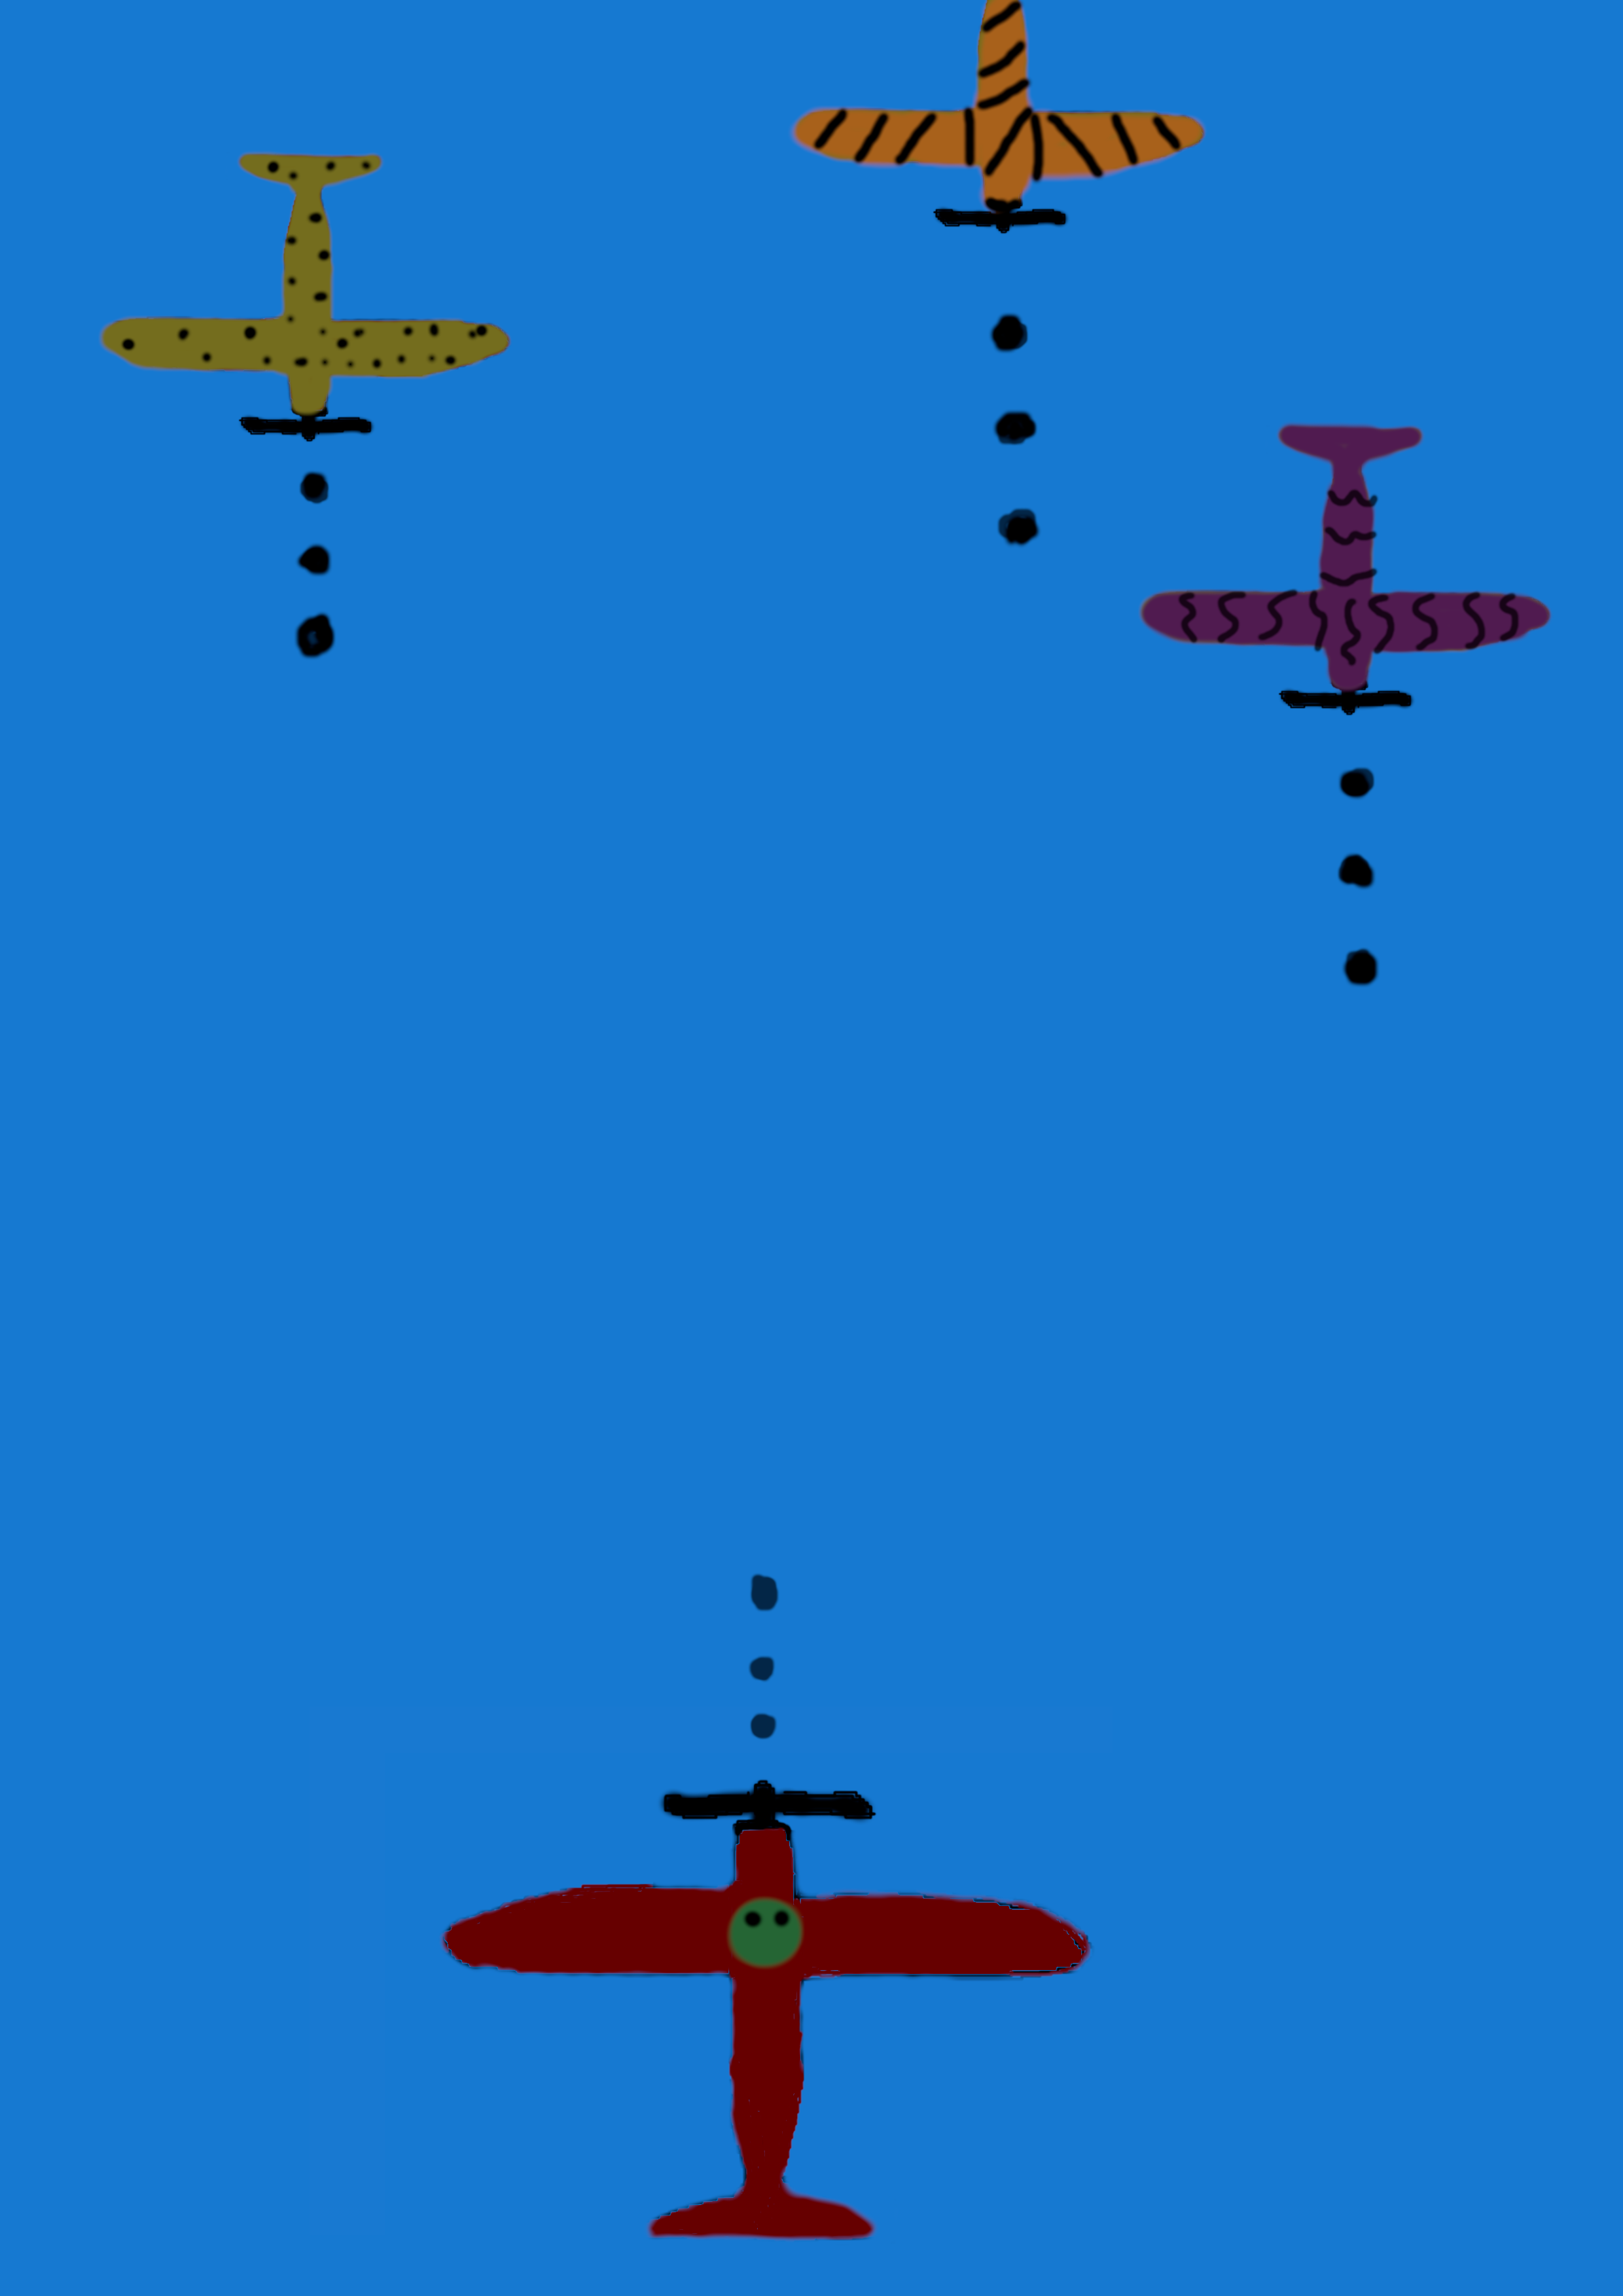
\includegraphics[width=5cm]{Dogeater.png}
  \caption{Spelaren(längst ner) slåss mot 3 fiender}
\end{figure}

\section{Kravformulering}
\subsection{Ska-krav}
\begin{enumerate}
  \item [1] Det ska finnas en spelare och minst en fiende per bana.
  \item [2] Spelaren ska kunna röra på sig och skjuta projektiler, se Tabell 1.
  \item [3] Det ska finnas olika typer av projektiler, se rubrik 3.4.
  \item [4] Det ska finnas olika fiendetyper, se rubrik 3.3. 
  \item [5] Fiender rör sig från toppen till botten av skärmen.
  \item [6] Fiender ska enbart kunna kollidera med spelaren projektiler och förstöras om de gör det.
  \item [7] När spelaren kolliderar med en fiende projektil eller en fiende så förlorar spelaren ett liv.
            Om spelaren inte har några liv kvar så börjar spelaren om banan från början.
  \item [8] En bana består av en tvådimensionell blå bakgrund.
  \item [9] Banan har en fixerad längd och om spelaren kommer till slutet så klarar spelaren banan och spelet stängts ner.
\end{enumerate}
\subsection{Bör-krav}
\begin{enumerate}
  \setcounter{enumi}{13}
  \item [10] Bakgrunden kan vara mycket mer detaljerad, med en textur som fortsätter i evighet.
  \item [11] Det ska finnas en boss vid slutet av vissa banor.
             Bossen kommer inte röra sig till botten av skärmen utan stannar tills den tagit nog med skada.
             Efter den har tagit nog med skada så vinner spelaren nivån.
  \item [12] Spelaren skall endast ta skada då piloten i spelarens flygplan kolliderar med en fientlig projektil eller enhet. Kontakt med resterande delar av stridsflygplanet räknas ej. 
  \item [13] Spelaren ska kunna skjuta olika slags projektiler med hjälp av ''powerups'', t.ex snabbare projektiler som gör mer skada.
  \item [14] Nya banor kommer vara låsta och behöva låsas upp genom att spelaren klarar de tidigare nivåerna. 
  \item [15] En enkel startmeny där spelaren kan välja bana.
  \item [16] När spelaren förlorar ett liv förstörs alla projektiler och spelaren blir immun mot skada under en kort tid.
  \item [17] En knapp som gör att spelaren rör sig mycket långsammare.
  \item [18] UI som visar hur många liv spelaren har.
  \item [19] Animationer för när fiender och spelaren förstörs.
  \item [20] En text som gratulerar spelaren att spelaren har avklarat banan.
  \item [21] Efter spelaren klarar en bana så skickas spelaren till nästa nivå.
\end{enumerate}
\section{Kravuppfyllelse}
\textbf{Spelet ska simulera en värld som innehåller olika typer av objekt. Objekten ska ha olika beteenden och röra sig i världen och agera på olika sätt när de möter andra objekt.}
\\
Täcks av kraven: 1, 3, 4, 5, 6, 7

\textbf{Det måste finnas minst tre olika typer av objekt och det ska finnas flera instanser av minst två av dessa. T.ex ett spelarobjekt och många instanser av två olika slags fiendeobjekt.}
\\
Täcks av kraven: 1, 3, 4\\
Det ska finnas ett spelarobjekt, projektilobjekt och ett fiendeobjekt.
Det kommer finnas olika instanser av fiende och projektil objektet.
\\\\
\textbf{Ett beteende som måste finnas med är att figurerna ska röra sig över skärmen. Rörelsen kan följa ett mönster och/eller vara slumpmässig. Minst ett objekt, utöver spelaren ska ha någon typ av rörelse.}
\\
Täcks av kraven: 3, 4, 5 
\\\\
\textbf{En figur ska styras av spelaren, antingen med tangentbordet eller med musen. Du kan även göra ett spel där man spelar två stycken genom att dela på tangentbordet (varje spelare använder olika tangenter). Då styr man var sin figur.}
\\
Täcks av kravet: 2 
\\\\
\textbf{Grafiken ska vara tvådimensionell.}
\\
Täcks av implementationen.
\\\\
\textbf{Det ska finnas kollisionshantering}
\\
Täcks av kraven: 6, 7 
\\\\
\textbf{Det ska vara enkelt att lägga till eller ändra banor i spelet}
\\
Täcks av implementationen.
\\\\
\textbf{Spelet måste upplevas som ett sammanhängande spel som går att spela!}
\\
Täcks av kravet: 9

\end{document}
